%
%-----------------------------------
\section{Strontium}
\label{eq:strontium}
%-----------------------------------
%

We estimate quantities from two strontium nMOTs. The first one, reproduced by Thomas Loftus \cite{loftus2004narrow} and his research group, was used to estimate quantities related to the atomic cloud profile. The second one was used to analyse temperature and was reproduced by the research group of the professor Raul C. Teixeira at Federal University of São Carlos. We shall call each experiments \textbf{Loftus nMOT} and \textbf{IFSC nMOT}, respectively. Both use the same electronic transition presented in Table \ref{tab:electronic-transition-St-loftus}, whose narrowness is $ \eta = 1.6 $ from equation (\ref{eq:narrowness}) and $ R = 15.8 $ from equation (\ref{eq:gravity-radiation-force-ratio}). Since these values are lower than the Dreon nMOT, it is easier to reach the power-broadened regime since the MOT forces will be much lower. Moreover, this transition is the same as the one analysed in Chapter \ref{ch:MOT} and therefore it does not depend on the spin-polarization phenomenon as the Dreon nMOT.

\begin{table}[ht!]
    \centering
    \caption{Electronic transition parameters from the Loftus nMOT and the IFSC nMOT.}
    \begin{tabular}{|c|c|c|}
        \hline
        \textbf{Symbol} & \textbf{Quantity} & \textbf{Value} \\ \hline
        $ \Gamma / 2\pi $ & Natural Linewidth & $ 7.5\ kHz $ \\
        $ \lambda $ & Resonant wavelength & $ 689\ nm $ \\
        $ J_{gnd} $ & Ground state angular momentum & $ 0 $ \\
        $ g_{gnd} $ & Ground state Landé factor & $ 0 $ \\
        $ J_{exc} $ & Excited state angular momentum & $ 1 $ \\
        $ g_{exc} $ & Excited state Landé factor & $ 1.5 $ \\
        $ m $ & Mass & $ 88\ u $ \\
        \hline
    \end{tabular}
    \vspace{10px}
    \legend{Source: LOFTUS \textit{et al}. \cite{loftus2004narrow}. TEXEIRA. \textit{et al}.}
    \label{tab:electronic-transition-St-loftus}
\end{table}

Both Loftus nMOT and IFSC nMOT have the same arrangement as shown in Section \ref{sec:three-dimensional-MOT}. The laser beam setup and the magnetic field profile are presented in Tables \ref{tab:loftus-laser-beams}, \ref{tab:Loftus-magnetic-field}, and \ref{tab:IFSC-magnetic-field}. The polarization of the laser beams in the gravity direction are different than the polarization of the other ones since the negative component of the magnetic field is in this direction.

\begin{table}[ht!]
    \centering
    \caption{Wave vector direction $ (x, y, z) $ and polarization $ (\sigma_+, \sigma_-, \pi) $ in the laboratory frame (see Section \ref{sec:magnetic-field-frame}) from the Loftus nMOT and the IFSC nMOT. The laser beams of the Loftus nMOT have the saturation parameter $ s_0 = 248 $ and waist $ w = 2.6\ cm $, whereas the laser beams of the IFSC nMOT have $ s_0 = 102 $ and $ w = 6.0\ cm$.}
    \begin{tabular}{|c|c|}
        \hline
        \textbf{Wave vector (arb. unit.)} & \textbf{Polarization} \\ \hline
        $ (1, 0, 0) $ & $ (1, 0, 0) $ \\
        $ (-1, 0, 0) $ & $ (1, 0, 0) $ \\
        $ (0, 1, 0) $ & $ (1, 0, 0) $ \\
        $ (0, -1, 0) $ & $ (1, 0, 0) $ \\
        $ (0, 0, 1) $ & $ (0, 1, 0) $ \\
        $ (0, 0, -1) $ & $ (0, 1, 0) $ \\
        \hline
    \end{tabular}
    \vspace{10px}
    \legend{Source: LOFTUS. \textit{et al}. \cite{loftus2004narrow}. TEXEIRA. \textit{et al}.}
    \label{tab:loftus-laser-beams}
\end{table}

\begin{table}[ht!]
    \centering
    \caption{Parameters of the magnetic field profile from the Loftus nMOT.}
    \begin{tabular}{|c|c|c|}
        \hline
        \textbf{Symbol} & \textbf{Quantity} & \textbf{Value} \\ \hline
        $ B_0 $ & Axial gradient & $ 10 G / cm $ \\
        $ B $ & Magnetic Field & $ B_0(\hat{x}/2 + \hat{y}/2 - \hat{z}) $ \\
        $ B_{bias} $ & Bias & $ 0 $ \\
        \hline
    \end{tabular}
    \vspace{10px}
    \legend{Source: LOFTUS. \textit{et al}. \cite{loftus2004narrow}.}
    \label{tab:Loftus-magnetic-field}
\end{table}

\begin{table}[ht!]
    \centering
    \caption{Parameters of the magnetic field profile from the IFSC nMOT.}
    \begin{tabular}{|c|c|c|}
        \hline
        \textbf{Symbol} & \textbf{Quantity} & \textbf{Value} \\ \hline
        $ B_0 $ & Axial gradient & $ 5 G / cm $ \\
        $ B $ & Magnetic Field & $ B_0(\hat{x}/2 + \hat{y}/2 - \hat{z}) $ \\
        $ B_{bias} $ & Bias & $ 0 $ \\
        \hline
    \end{tabular}
    \vspace{10px}
    \legend{Source: TEXEIRA. \textit{et al}.}
    \label{tab:IFSC-magnetic-field}
\end{table}

%-----------------------------------
\subsection{Atomic cloud profile}
\label{sec:cloud-profile-dysprosium}
%-----------------------------------

The in-situ and estimated atomic cloud profiles from the Loftus nMOT are shown in Figures \ref{fig:Loftus-in-situ-atomic-cloud-profile} and \ref{fig:Loftus-simulated-atomic-cloud-profile}. They are similar to the Dreon profiles, as discussed in Section \ref{sec:cloud-profile-dysprosium}, but the eccentricities of the Loftus profiles are larger than those of the Dreon since the MOT forces are smaller. Moreover, the ellipsoid that bounds the atomic cloud is more clear for the Loftus nMOT, such that its bottom is clearly visible. Overall, the Loftus nMOT exhibits the properties of power-broadened nMOTs more clearly than the Dreon nMOT due to its smaller narrowness.
\begin{figure}[!ht]
    \centering
    \begin{subfigure}[b]{0.58\linewidth}
        \centering
        \subcaption{Estimated atomic cloud profile.}
        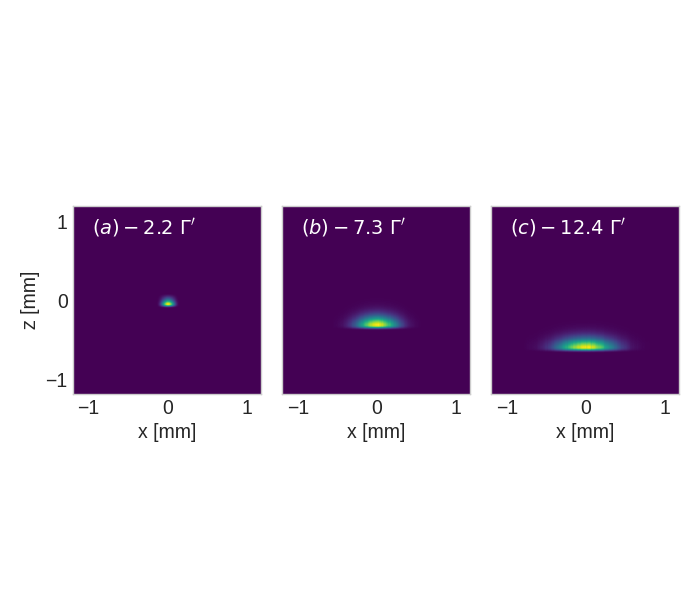
\includegraphics[width=\textwidth]{USPSC-img/sr_loftus_cloud_profile.png}
        \label{fig:Loftus-simulated-atomic-cloud-profile}
    \end{subfigure}
    \hfill
    \begin{subfigure}[b]{0.38\linewidth}
        \centering
        \subcaption{In situ atomic cloud profile.}
        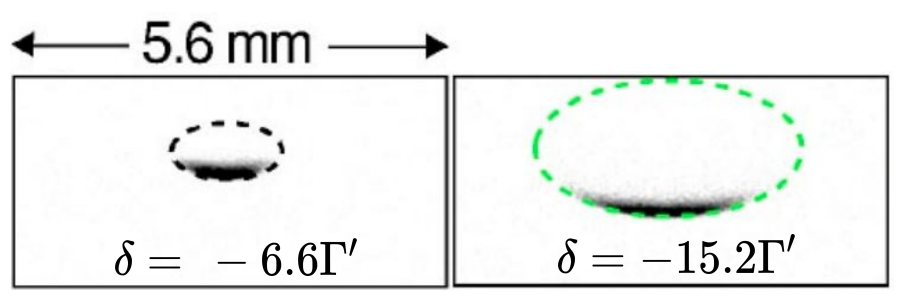
\includegraphics[width=\textwidth]{USPSC-img/loftus-atomic-cloud-profile.png}
        \vspace{40px}
        \label{fig:Loftus-in-situ-atomic-cloud-profile}
    \end{subfigure}
    \caption{(a) Estimated atomic cloud profile for different laser detunings based on equation (\ref{eq:joint-position-distribution}). (b) In-situ atomic cloud profiles from the Loftus nMOT.}
    \legend{Source (a): By the author; (b): LOFTUS. \textit{et al}. \cite{loftus2004narrow}.}
\end{figure}

The theoretical centre of mass given by equation (\ref{eq:centre-of-mass-power-broadened-regime}) fits perfectly the estimated values roughly about $ \Delta = -5\Gamma' $, as shown in Figure (\ref{fig:sr-centre-of-mass}). For laser detunings roughly below $ 5\Gamma' $ in module, we consider that nMOT is not in the power-broadened regime. Both estimated and theoretical centre of mass are about $ 0.1 mm $ above the experimental measures.

\begin{figure}[!ht]
    \centering
    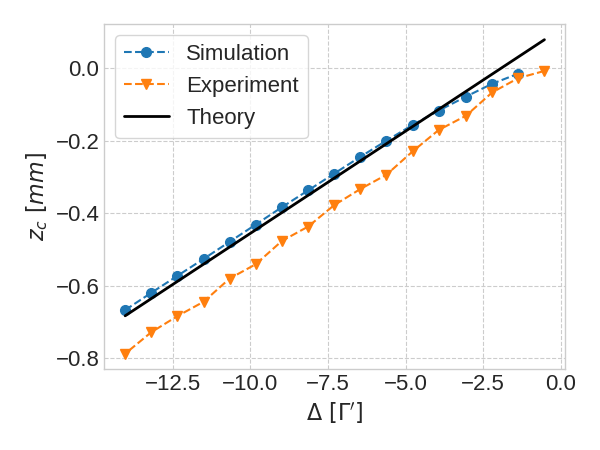
\includegraphics[width=0.5\textwidth]{USPSC-img/sr_centre_of_mass.png}
    \vspace{5px}
    \caption{Centre of mass as a function of the laser detunings from the Loftus nMOT. The blue spheres, orange triangles, and black line are the estimated, experimental, and theoretical centre of mass respectively.}
    \legend{Source: By the author.}
    \label{fig:sr-centre-of-mass}
\end{figure}

We do not find experimental measures of the cloud size from the Loftus nMOT. Nevertheless, we obtained the cloud sizes based on equation (\ref{eq:simulated-cloud-sizes}), as illustrated in Figure \ref{fig:sr-loftus-cloud-size}. The $x$ and $y$ cloud size components is essentially the same since the MOT force are symmetrical in these directions. The the larger the laser detuning module, the more spread the atomic cloud is in the directions perpendicular to the gravity. The $z$ component of the cloud size has a different behaviour. Roughly about $ \Delta = -6\Gamma' $, $ \sigma_z $ becomes constant $ -0.5nm $.

\begin{figure}[!ht]
    \centering
    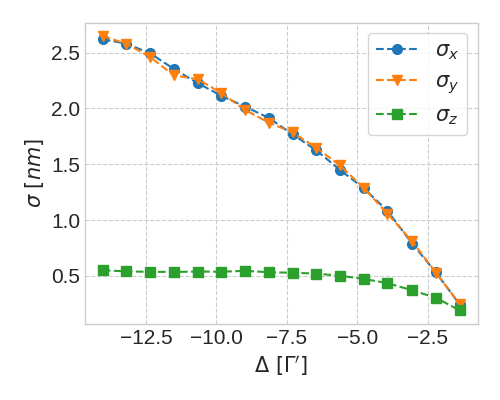
\includegraphics[width=0.48\textwidth]{USPSC-img/sr_loftus_cloud_size.png}
    \vspace{5px}
    \caption{Cloud sizes components from the Loftus nMOT as a function of the laser detuning. The blue spheres, orange triangles, and green squares are the estimated $ x $, $ y $, and $ z $ cloud size components respectively.}
    \legend{Source: By the author.}
    \label{fig:sr-loftus-cloud-size}
\end{figure}


%-----------------------------------
\subsection{Temperature}
\label{temperature}
%-----------------------------------

We simulate two sets of temperatures presented in Figures \ref{fig:IFSC-temperature-detuning} and \ref{fig:IFSC-temperature-detuning} by fixing either the saturation parameter or the laser detuning. In the first one, for detunings roughly smaller than $ -4 \Gamma' $, the experimental temperatures increases with the laser detuning whereas the estimated values decrease, as the Dreon nMOT. Therefore, in this range, the nMOT is not in the power-broadened regime. In the complementary range, the estimated temperature is approximately constant and equals to $ 4 \mu K $ whereas the experimental temperatures slowly increases from $ 4\mu K $ to $ 5.5\mu K $ so that the maximum divergence is $ 1.5\mu K $. The theoretical temperature given by equation (\ref{eq:Doppler-temperature-high-saturation}) is $ 1.8 \mu K $, which is smaller than both estimated and experimental values. In the second set of temperatures, for saturation parameters roughly smaller than $ 450 $, the maximum divergence is $ 1 \mu K $, whereas for the complementary range, the maximum divergence increases to $ 6\mu K $. In both sets of temperatures, the experimental values are closer to the estimated values than the theoretical ones.

\begin{figure}[!ht]
    \centering
    \begin{subfigure}[b]{0.48\linewidth}
        \centering
        \subcaption{Temperature vs. laser detuning.}
        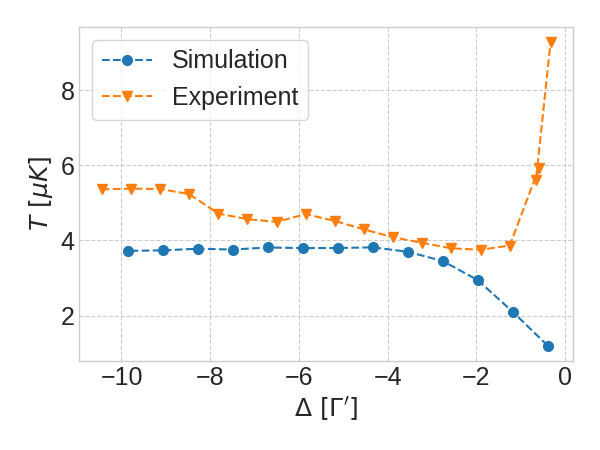
\includegraphics[width=\textwidth]{USPSC-img/sr-ifsc-temperature_vs_detuning.png}
        \label{fig:IFSC-temperature-detuning}
    \end{subfigure}
    \hfill
    \begin{subfigure}[b]{0.48\linewidth}
        \centering
        \subcaption{Temperature vs saturation parameter.}
        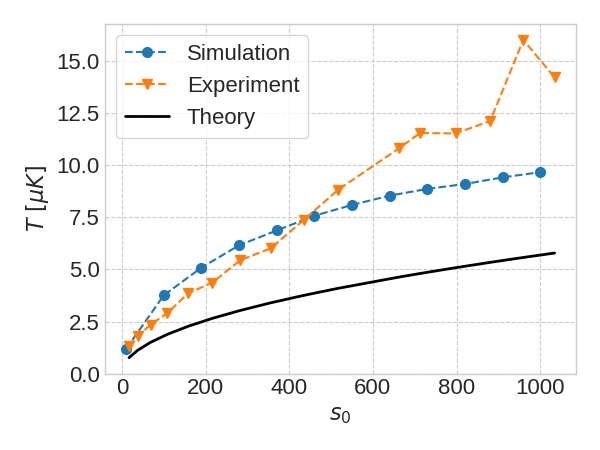
\includegraphics[width=\textwidth]{USPSC-img/sr_ifsc_temperature_vs_saturation.png}
        \vspace{10px}
    \end{subfigure}
    \caption{(a) Temperature as a function of the laser detuning for a saturation parameter of $ s = 102 $. (b) Temperature as a function of the saturation parameter for a laser detuning of $ \delta = -3.1\ MHz $. The blue spheres and orange triangles are the estimated and experimental values from the IFSC nMOT respectively.}
    \legend{Source: By the author.}
\end{figure}
